\documentclass[11pt]{article}
\usepackage[margin=0.9in]{geometry}
\usepackage[T1]{fontenc}
\usepackage{lmodern}
\usepackage{graphicx}
\usepackage{booktabs}
\usepackage{float}
\usepackage{xcolor}
\usepackage{array}
\usepackage{tabularx}
\usepackage{url}
\usepackage[hidelinks]{hyperref}

\setlength{\parindent}{0pt}
\setlength{\parskip}{5pt}
\newcommand{\figwidth}{0.98\linewidth}

\title{\vspace{-1.4cm}EE291F Homework 2\\[2pt]
DC and Formality Flow for MohoTop (RISC-V)}
\author{Jichen Zhou\\Student ID: 2603000020}
\date{November 18, 2026}

\begin{document}
\maketitle

\section{Objective}

Run the three-stage Synopsys Design Compiler flow for \texttt{MohoTop}, export
the synthesized netlist, SDC, SDF, and reports, and use Formality to prove that
the DC netlist is logically equivalent to the original RTL.

\section{Environment and Inputs}

\begin{table}[H]
\centering
\small
\begin{tabular}{@{}ll@{}}
\toprule
Item & Value \\
\midrule
Top module & \texttt{MohoTop} (RV32I, five-stage pipeline) \\
Clock & \texttt{io\_pins\_clk}, 6.667 ns (150 MHz) \\
Reset & \texttt{io\_pins\_rst} \\
Memories & 2 $\times$ \path{mem_hl55_2048x32_sp_m1} \\
Technology & HL055P\_7M6X1T4\_RDL, RVT + LVT standard cells \\
Process library & \path{/mnt/nfs_share/EE291F/3003/tech.prj} \\
DC tool & Synopsys Design Compiler R-2020.09-SP5 \\
Formality tool & Synopsys Formality S-2021.06 \\
\bottomrule
\end{tabular}
\end{table}

The RTL and SDC were copied unchanged from the course project. The clock period
is 6.667 ns in both DC and the exported SDC; the final stage restores the
original 0.50 ns uncertainty before exporting. The three DC stages completed
successfully, and Formality used the final DC netlist and the original RTL.

\section{DC Synthesis Flow}

\begin{table}[H]
\centering
\small
\begin{tabular}{@{}lll@{}}
\toprule
Stage & Command & Generated files \\
\midrule
01 elaborate & \texttt{make dc-elaborate} & \path{MohoTop.ddc}, \texttt{netlist.v}, \path{MohoTop.svf} \\
02 compile & \texttt{make dc-compile} & \path{MohoTop.ddc}, \texttt{netlist.v}, \path{MohoTop.svf} \\
03 final & \texttt{make dc-final} & \path{dc/MohoTop_syn.v}, \texttt{.sdc}, \texttt{.sdf}, three reports \\
\bottomrule
\end{tabular}
\end{table}

The figures below are terminal transcripts rendered from the recorded run logs;
each shows the command, the main tool activity, and the success message.

\subsection{Stage 01: Elaborate}

The RTL was analyzed and elaborated with the HL55 libraries, and the clock and
reset networks were protected with \texttt{set\_dont\_touch\_network}. The run
took about 67 s and generated \path{MohoTop.ddc}, \texttt{netlist.v}, and the
SVF for Formality.

\begin{figure}[H]
\centering
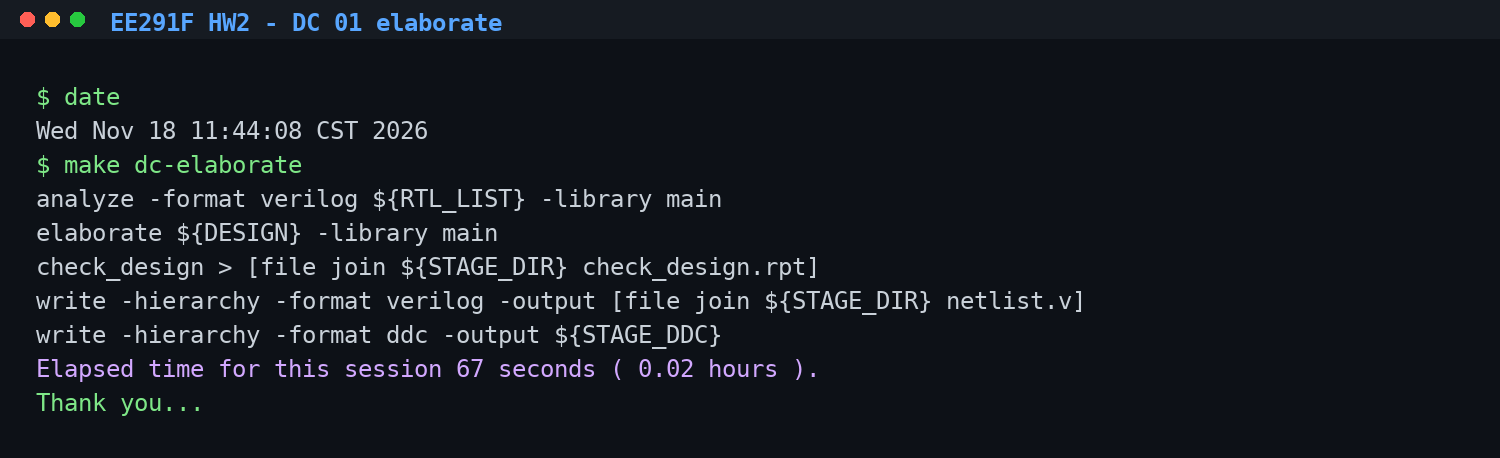
\includegraphics[width=\figwidth]{figures/stage_dc_elaborate.png}
\caption{DC elaborate: analyze, elaborate, check\_design, and DDC export.}
\end{figure}

\subsection{Stage 02: Compile}

The design database was restored, the SDC was read, and \texttt{compile\_ultra}
mapped the design to the HL55 standard cells. The run took about 453 s and
generated the compiled \path{MohoTop.ddc}, \texttt{netlist.v}, and a second SVF.

\begin{figure}[H]
\centering
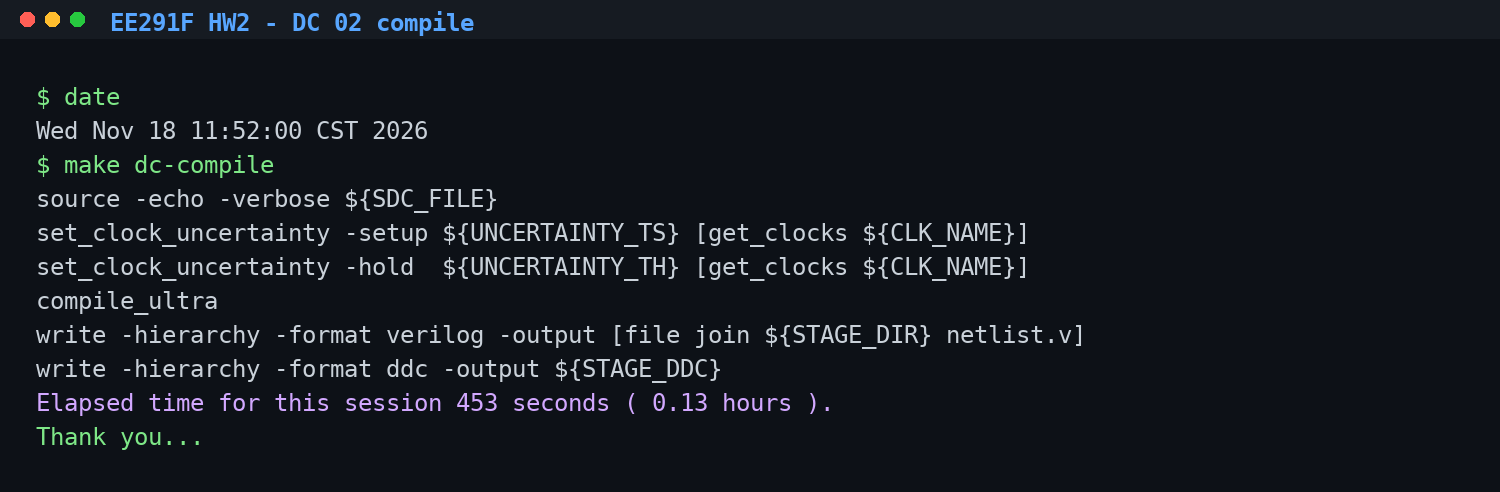
\includegraphics[width=\figwidth]{figures/stage_dc_compile.png}
\caption{DC compile: SDC source, compile\_ultra, and netlist export.}
\end{figure}

\subsection{Stage 03: Final}

The compiled database was restored, the original 0.50 ns uncertainty was
applied, and the final netlist, SDC, SDF, and QoR/timing/area reports were
written. The files were copied into the \path{dc/} submission directory.

\begin{figure}[H]
\centering
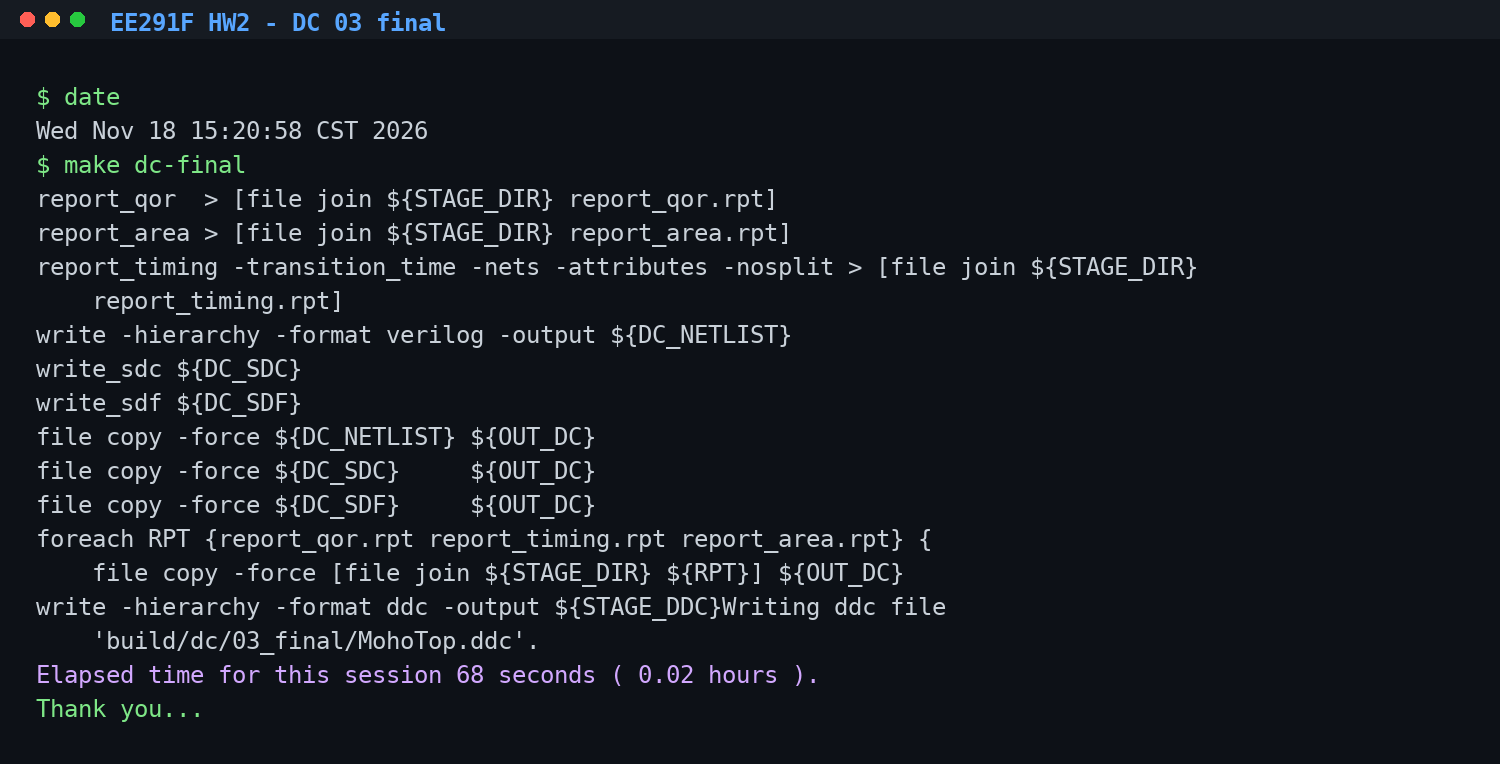
\includegraphics[width=\figwidth]{figures/stage_dc_final.png}
\caption{DC final: reports, netlist/SDC/SDF export, and deliverable copy.}
\end{figure}

\section{Formality Verification}

Formality read the original RTL as the reference, the final DC netlist as the
implementation, and the two SVF files produced by the elaborate and compile
stages. Auto setup was enabled. The verification result is shown below.

\begin{figure}[H]
\centering
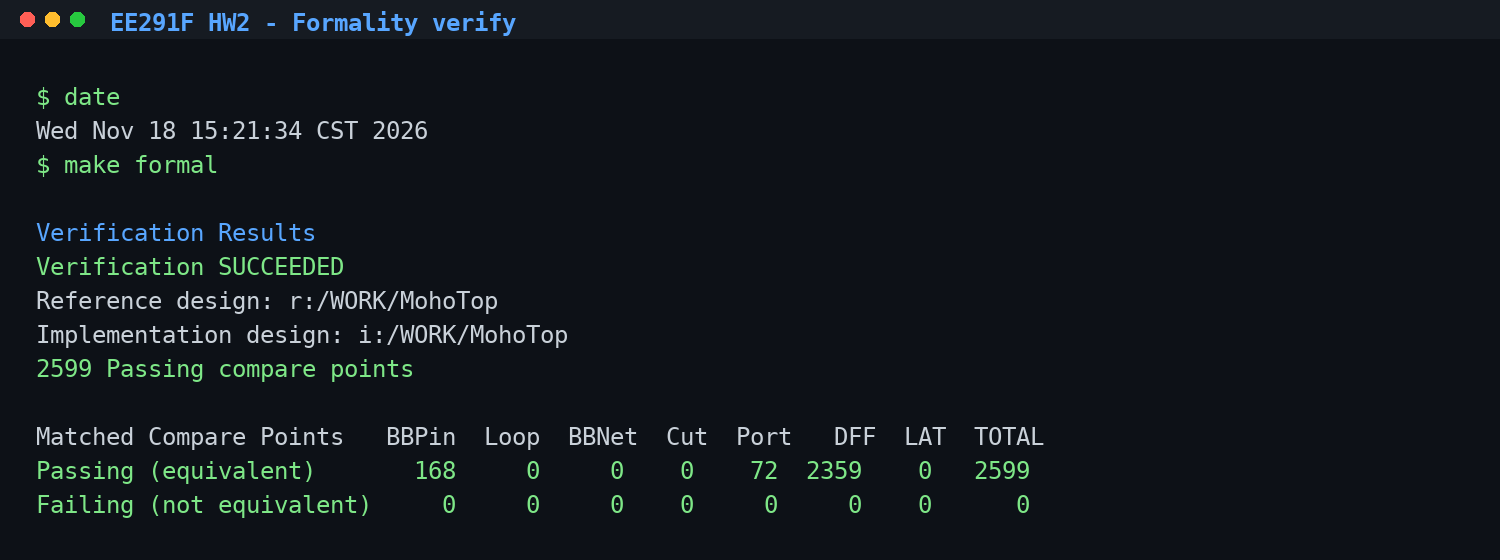
\includegraphics[width=\figwidth]{figures/formal_verify.png}
\caption{Formality verify result: 2599 passing and 0 failing compare points.}
\end{figure}

Verification \textbf{SUCCEEDED}: 2599 compare points passed and 0 failed. The
unmatched report lists 32 reference-only DFFs, all
\path{stageD/rf_u/regs_0_reg[0..31]}; this is the RISC-V \texttt{x0} register
entry, which is constant in the implementation, so these flops are optimized
away. There are no implementation-only unmatched points. The two memories are
treated as black boxes:

\begin{itemize}
\item \path{topArea_soc/ram_u/core_u/sramHl55_2/u}
\item \path{topArea_soc/rom_m/core_u/sramHl55_2/u}
\end{itemize}

Both are \path{mem_hl55_2048x32_sp_m1} macros, which is allowed by the
assignment. Formality wrote the four required reports:
\path{report_guidance.rpt}, \path{report_failing_points.rpt},
\path{report_unmatched_points.rpt}, and \path{report_black_boxes.rpt}. The
guidance report shows 421 accepted SVF commands, 0 rejected.

\section{Final Deliverables}

The final \texttt{ls -lh} listing is shown below. The netlist, SDC, SDF, and all
reports are non-empty and come from the same complete run.

\begin{figure}[H]
\centering
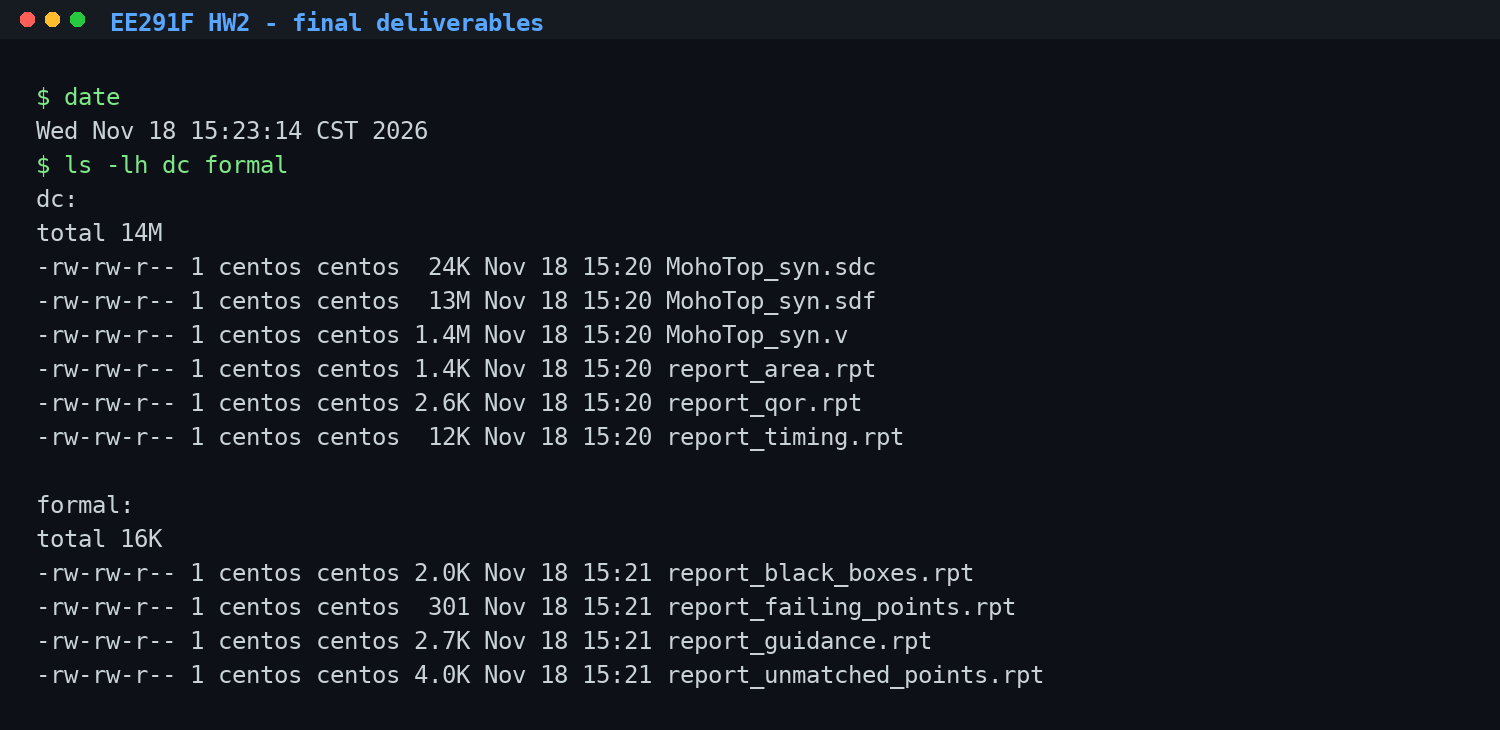
\includegraphics[width=\figwidth]{figures/deliverables.png}
\caption{Final \texttt{ls -lh dc formal} output.}
\end{figure}

\begin{table}[H]
\centering
\small
\begin{tabular}{@{}llr@{}}
\toprule
Directory & File & Size \\
\midrule
\texttt{dc/} & \path{MohoTop_syn.v} & 1.4 MB \\
\texttt{dc/} & \path{MohoTop_syn.sdc} & 24 KB \\
\texttt{dc/} & \path{MohoTop_syn.sdf} & 13 MB \\
\texttt{dc/} & \path{report_qor.rpt} & 2.6 KB \\
\texttt{dc/} & \path{report_timing.rpt} & 12 KB \\
\texttt{dc/} & \path{report_area.rpt} & 1.4 KB \\
\texttt{formal/} & \path{report_guidance.rpt} & 2.7 KB \\
\texttt{formal/} & \path{report_failing_points.rpt} & 301 B \\
\texttt{formal/} & \path{report_unmatched_points.rpt} & 4.0 KB \\
\texttt{formal/} & \path{report_black_boxes.rpt} & 2.0 KB \\
\bottomrule
\end{tabular}
\end{table}

\section{Timing and Area Results}

DC reports setup timing as met (0 violating paths). The critical path slack is
+1.00 ns. Hold has 25 small violations, worst $-0.02$ ns and total $-0.20$ ns;
these are normally fixed in place-and-route and are reported here for
completeness.

\begin{table}[H]
\centering
\small
\caption{DC final QoR.}
\begin{tabular}{@{}lr@{}}
\toprule
Metric & Value \\
\midrule
Setup WNS & 0.00 ns \\
Setup TNS & 0.00 ns \\
Setup violating paths & 0 \\
Critical path slack & +1.00 ns \\
Hold violating paths & 25 \\
Worst hold slack & $-0.02$ ns \\
Total hold violation & $-0.20$ ns \\
\bottomrule
\end{tabular}
\end{table}

\begin{table}[H]
\centering
\small
\caption{Area and instance counts from \texttt{report\_area.rpt}.}
\begin{tabular}{@{}lr@{}}
\toprule
Metric & Value \\
\midrule
Combinational area & 21{,}487.752 \\
Noncombinational area & 18{,}646.524 \\
Buffer/inverter area & 1{,}389.492 \\
Macro/black-box area & 108{,}090.227 \\
Total cell area & 148{,}224.502 \\
Leaf cells & 12{,}257 \\
Sequential / combinational & 2{,}361 / 9{,}896 \\
Macros / black boxes & 2 \\
\bottomrule
\end{tabular}
\end{table}

\section{Conclusion}

All three DC stages completed successfully, and Formality proved the final
netlist equivalent to the RTL with 2599 passing and 0 failing compare points.
The two SRAM macros are the only black boxes. The required \texttt{dc/} and
\texttt{formal/} deliverables are complete and non-empty.

\end{document}